\section{WURC Array 8x8}
\label{sec_wurc_8x8}

	Once we had demonstrated basic \ac{MU-MIMO} feasibility using the experimental 4x4 \ac{SDR} platform in Section~\ref{sec_wurc_4x4}, the next step was to leverage the modular design of \ac{WURC} and develop a more integrated platform suitable for scaling the beamforming performance of the system.
	
\begin{figure}[p] % WURCLab MIMO Node
\centering
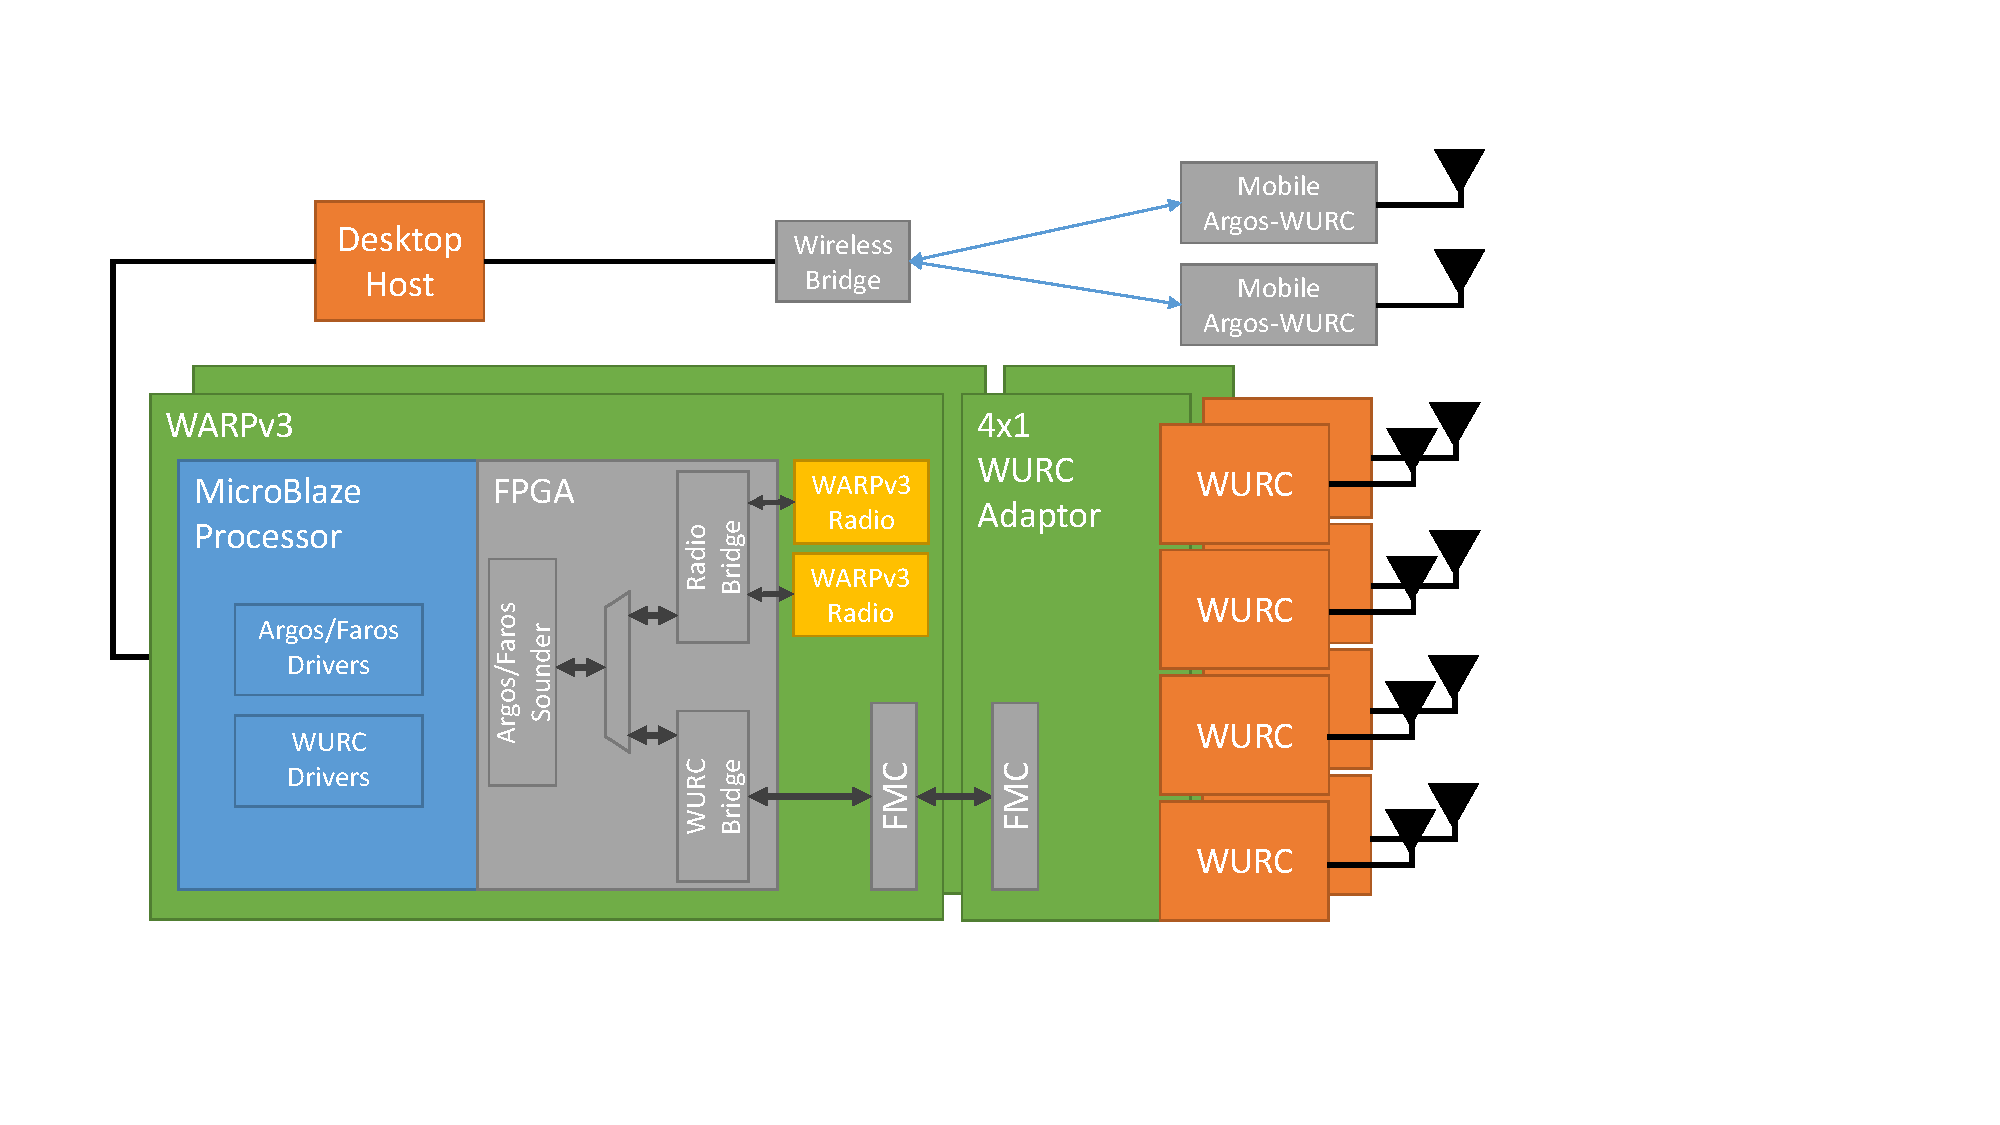
\includegraphics[width=1\linewidth]{./figs/argos-wurc_system_diagram}
\caption{System diagram of the $8\times8$ WURC \ac{AP} and mobile \acp{STA}.}
\label{fig:wurc_argos_hw}
\end{figure}


\begin{figure}[p] % WURCLab MIMO Node
\centering
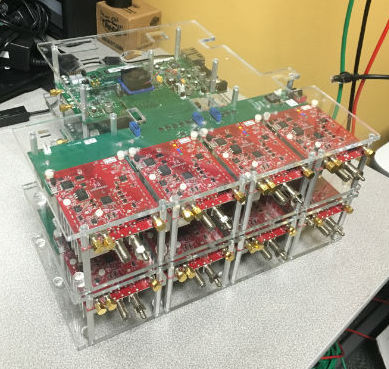
\includegraphics[width=0.7\linewidth]{./figs/MIMO_node.jpg}
\caption{Photo of the implemented $8\times8$ WURC \ac{AP} for UHF-band operation.}
\label{fig:mimohw}
\end{figure}

	Although \ac{MU-MIMO} capabilities are available on ``wave-two'' 802.11ac \ac{ASIC} chips, the research community has been limited by the lack of cross-layer observability and access that can be had on commodity hardware, making experimentation with \ac{MU-MIMO} systems difficult.
 In addition, to the best of our knowledge, no 802.11af \acp{ASIC} has yet been announced, and certainly not one that implements the maximum 4-stream with 8-transmit antennas, 8x1x1x1x1 \ac{MU-MIMO} beamforming allowed in the 802.11 standard \cite{std11af}.
 For that reason, we developed the hardware and software stack of a custom \ac{SDR} platform that allows us to arbitrarily generate, intercept, and modify \ac{MU-MIMO} transmissions that are designed to be 802.11af-compatible with 8x1x1x1x1 operation.
	In this section we discuss the architectures and challenges involved in designing and scaling our \ac{WURC}-based \ac{MU-MIMO} platform.
	
\subsection{Hardware Platform Design}
\label{sec:wurc_argos_design}

%We further extend the \ac{WURC} UHF test equipment that we developed in previous sections for rapid physical-layer prototyping in UHF bands \cite{anand2014case, WURC}.
	%\ac{WURC} was designed to enable high-power transmission up to 1~W and reception of wide-band radio signals in frequencies between 470-698~MHz \cite{WURC} and each module provides one complete analog radio chain for use with a single WARPv3 \ac{SDR} baseband \cite{warpProject}.
	%Multiple WARPv3 boards can be clock synchronized with a daisy-chained reference clock and shared sampling trigger.

	The equipment and daisy-chain topology for the 4x4 system in Figure~\ref{fig_wurc_4x4_sys_diagram} suffers from two key impairments that limit the scalability of the hardware.
	First, the system utilizes a daisy-chain clocking topology that introduces additional transmission and reception phase errors and aperture jitter as the reference clock signal is forwarded \cite{kester2008aperture}.
	The timing error introduced on each hop due to clock skew and system noise can be viewed as a zero-mean Gaussian random process where the variance of the aggregate Gaussian random process sampled at each hop increases proportionally to the number of hops.
	As the system scales from 4x4 to 8x8 and more, a daisy-chained clocking structure becomes more difficult to maintain, particularly when each interconnect is cabled and prone to damage or disconnect during transport and setup.
	
	In addition, the topology in Figure~\ref{fig_wurc_4x4_sys_diagram} also requires the sharing of a timing synchronization trigger that also suffers from signal bi-stability caused by signals crossing from one clocking domain to the next \cite{cummings2008clock}.
	When a bi-stable trigger falls on a different cycle of the destination clock in a coherent \ac{MIMO} system, it looks like a shift in channel phase equal to a full clock sampling period, and significantly disrupts coherent beamforming.
	This is a problem that can be managed in smaller-scale systems but requires more engineered solutions for large-scale systems.

	In order to address these issues and support modular, scalable, and mobile \ac{MIMO} \ac{SDR} arrays, we design, layout, and manufacture a clock-synchronized 4-radio adapter board that can connect up to 4 \ac{WURC} radio front-ends to a single WARPv3 baseband board (Fig.~\ref{fig:wurc_argos_hw}: the $4\times1$ WURC Adapter).
	With this architecture, RF reference clocks are now buffered and distributed in a tree topology, while inter-radio triggering is no longer needed since all data streams come from the same \ac{FPGA} and same clock domain.
	This has the added advantage of reducing the cost and hardware footprint of a 4-radio UHF \ac{AP} by eliminating extraneous WARPv3 boards compared to the previous design.
	
	To support the newly developed adaptor hardware, we develop the WARPLab software support (FPGA HDL, MicroBlaze C, and WARPLab extensions in MATLAB) to transparently integrate the four UHF radio front-ends with the existing WARPLab version 7.4 framework \cite{warpProject}, expanding upon the initial integration presented in Section~\ref{sec_warplab}.

\subsubsection{Antennas.}
\label{sec_8x8_antennas}

	Our over-the-air experiments utilize omni-directional 3~dBi August DTA240 portable UHF antennas for the \ac{AP}, mobile \acp{STA}, and indoor \acp{STA} while the static outdoor \acp{STA} use Comtelco Y42400WB 7~dBi log-periodic antennas.
	During experiments, the \ac{AP} antennas are configured in a linear array separated by a minimum of $\lambda/2$ distance to ensure sufficient de-correlation of the received signals.


%\subsubsection{Wireless Mobility.}
%\label{sec_8x8_backhaul}
%
	%Another key upgrade to the experimental design o
	%
	%\cite{shepard2015faros}

